\documentclass{article}
\usepackage[utf8]{inputenc}
\usepackage{graphicx}
\usepackage{hyperref}

\title{Satellite Object Recognition Using Remote Sensing Data}
\author{John Dinh, Collin Kennedy, Yunzhe Zhu}
\date{Due: 5/8/2022}

\begin{document}

\maketitle

\section{Project Proposal}

The goal of this project will be to do a big data analysis using remote sensing data to perform satellite image classification tasks. A few key algorithms and methods that would be appropriate are random forests, support vector classifiers, and decision trees.


\subsection{Big Data Analysis}

The vast majority of machine learning algorithms are designed to solve relation building and classification problems. With the continuous development and improvement of remote sensing satellite imagery in the geographical field, satellite imagery data is increasingly characterized by a large amount of data and high complexity. Therefore, in the past few decades, the geographic field has been trying to apply stronger and more effective machine learning methods to the tasks of information extraction and object recognition from remote sensing data. Between basic correction and processing of remote sensing data and advanced analytical applications of remote sensing data, there is often a classification of feature types. From the perspective of classification accuracy, the random forest classifier in the traditional machine learning field typically performers better than other classification methods, however, other algorithms such as SVM and decision trees will be considered as well. 

This project intends to use Landsat satellite data, which is most commonly used in the field of remote sensing. Among them, the 'Landsat ARD' dataset integrated in recent years has undergone most of the data pre-processing and is ideal test data \href{https://earthexplorer.usgs.gov/}{download from here}. In order to verify our data results and to extract training samples more easily, we use the USDA classification results for North American features as a reference and training data source \href{https://nassgeodata.gmu.edu/CropScape/}{download from here}. In order to reduce the difficulty of the project, we expect to tentatively set the experimental data range in three counties around Sacramento. If we make good progress, we can also do some experiments in the direction of a bigger data, set such as classifying satellite imagery of the whole of California or classifying the types of land objects in the whole of America.

\begin{figure}
  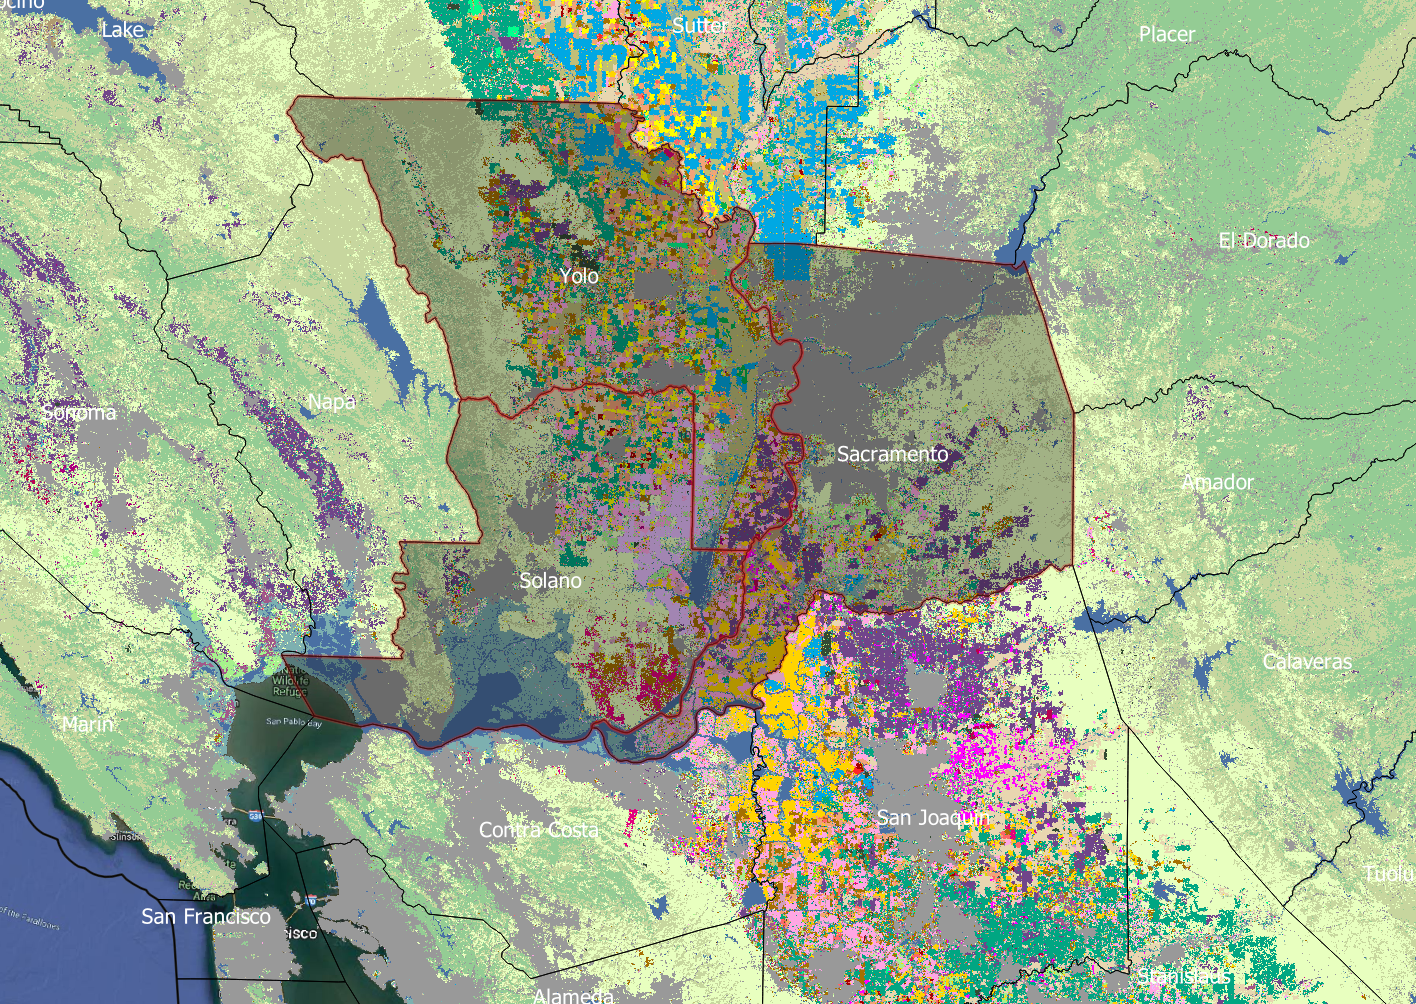
\includegraphics[width=\linewidth]{DataMap.png}
  \caption{California classification map with presupposed study area.}
  \label{fig:boat1}
\end{figure}

\subsection{Other considerations}
The most challenging aspect of the project will be to understand all the foundations that each respective classification method builds itself upon. For example, since the random forest is a substantial extension of bagging, a strong theoretical understanding of bootstrap estimation, boosting, and decision trees will be needed. Understanding these nuances will also provide a deeper understanding of this ensemble method. Another example of this is to see how regularization behaves on remote sensing data, which will particularly become useful when fitting a support vector classifier. Simply put, a challenge in this project will be observe how each variation of model of each algorithm performs given that we are using remote sensing data. 
\end{document}
